\section{Introduction}

Sematic Specification Framework for actor-based languages

Framework:
constant: Reuse the framework ...
inherit the rules of Timed Rebeca ... ABS 

Variable: policies - arguments ...
(Future and things that we did not consider)

When designing a new language: points of decision 

proving different theorems

The computational model of actors \cite{Hewitt77,Agha90} has been introduced to model concurrent and distributed systems. Such modeling has become very popular in practice. Scala programming language supports actor-models. Actors, the primitives of computation, are independent, well encapsulated, and of course, run concurrently. Each actor has its own variables, and its encapsulation prohibits other actors from accessing its variables directly. Each actor communicates with others only through message passing and owns a mailbox with a unique address to store the received messages. An actor's behavior is defined in terms of a set of message handlers that specify how the actor reacts upon processing each received message. In this model, message delivery is guaranteed but is not in-order; if an actor sends two messages to a destination, they will be received in any order. This assumption implicitly abstracts away from the effects of the network, i.e., delays over different routing paths, message conflicts, etc., and consequently makes it a suitable modeling framework for concurrent and distributed applications. 


Many different formal modeling languages, like ABS \cite{ABS}, Timed Rebeca \cite{SirjaniK16}, Lingua Franca, have been proposed based on this computational model (see also \cite{survay}). Each language considers a set of policies on the delivery/processing of messages or their maintenance in the buffers. These policies may depend on the domain of systems and network settings. Different network settings like Ethernet, wireless, CAN bus, etc. have different effects on how messages are dispatched among entities in a distributed system. Different policies on the receipt of messages, e.g., overwriting old messages, dropping when the buffer is overflow, etc., or taking messages from the buffer regarding the priority or timestamps of messages have been considered in these languages. These policies are not explicitly explained in the definition of languages and their effects can be only followed up in the semantic rules of languages. However, one can not easily understands from the semantic rules the set of policies considered in the language. %leading to those assumptions of semantic rules. 


%For the verification of distributed systems with the model checking technique, different aspects of systems like configuration of actors, timing or probabilistic aspects, and coordination are considered to define the behavior of the systems. The rules focusing on these aspects are interweaved by those assumptions on the networks and policies of message handlers. 
To have a precise comprehension of a language policies, we aim to provide a semantic specification framework for actor-based languages by which such policies are %each separate concern is 
explicitly identified. Our framework provides a set of template rules that their assumptions may need to be adjusted with regard to the policies and network settings. We explicitly identify those assumptions that show a policy. Each policy explicitly reveals a decision point in realization of the actor model leading to variation of languages. We have defined the rules based on the interaction between two actors and network to realize a point-to-point communication between actors. To capture the policies at the buffer level, we also consider the interaction between actors/network and their buffers. We consider three phases for a point-to-point message communication as illustrated in Figure \ref{Fig::schema}: 
\begin{itemize}
\item\textit{Sending}: Actors push their messages into the buffer of the abstract network entity. %The properties of the network settings defines how the message is added to the local state of the network. %At this phase the reliability is considered. 

\item\textit{Transferring}: The abstract network entity delivers messages from its buffer to the receiver. %In this phase, the affect of network setting is considered as reliable/unreliable delivery, the delay of messages, variations at message delivery such as  in-order, out-of-order, or causal-order delivery, scheduling of messages arrived at the same time, etc.

%\item\textit{Receiving}: The abstract network entity pushes the messages from the network buffer into the buffer of receivers. %The policies of the receiver on handling buffer overflow, overwriting old messages or dropping redundant messages are considered at this phases. 

\item\textit{Taking}: The actor chooses a message from the buffer to process it. %Policies at this phase realizes the buffer management concerns from the point-view of the application. It may consider the time-stamp or the priority of messages to defined which message should be processed at first.  
	
\end{itemize}

\begin{figure}[htbp]
	\centering
	\usetikzlibrary{shapes,positioning,decorations.pathmorphing}

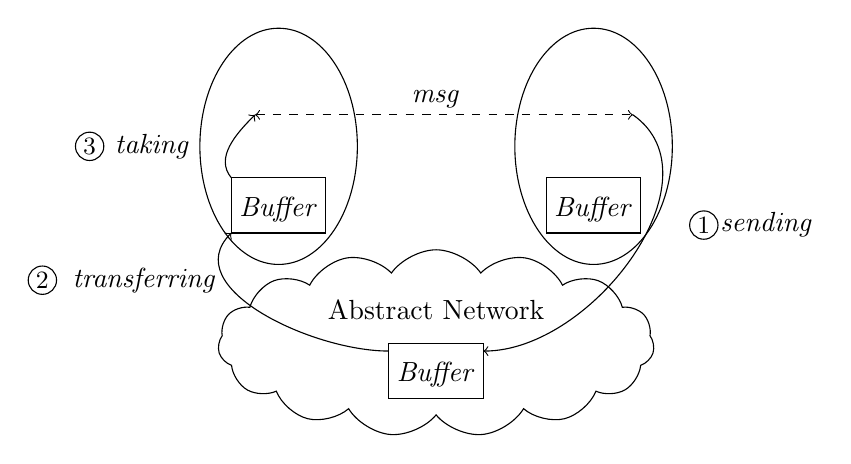
\begin{tikzpicture}%[arrow/.style = {draw=#1,-{Stealth[]}, shorten >=1mm, shorten <=1mm}]

\draw  (0,2.5) ellipse (1 and 1.5);
\draw  (-0.6,2.1) rectangle (0.6,1.4);
\node at (0,1.7) {$\it Buffer$};

\draw  (4,2.5) ellipse (1 and 1.5);
\draw  (3.4,2.1) rectangle (4.6,1.4);
\node at (4,1.7) {$\it Buffer$};

\draw[<->,dashed] (-0.3,2.9) -- (4.5,2.9) ;
\node at (2,3.1) {$\it msg$};

 \node[cloud, draw, align=left, cloud puffs=15,cloud puff arc=110, aspect=3, inner sep=1mm] at (2,0) {Abstract Network\\ \\};
 \draw  (1.4,0) rectangle (2.6,-.7);
\node at (2,-0.4) {$\it Buffer$};
 \draw[->] (4.5,2.9) to [out=-35, in=0] (2.6,-.1);%(4.6,0.4);
% \draw[->] (4.7,0.4) to [out=200, in=-20] (-0.7,0.3);
 \draw[->] (1.4,-0.1) to [out=180, in=225] (-0.6,1.4);
 \draw[->] (-0.6,2.1) to [out=130, in=225] (-0.3,2.9);
 
 \node[shape=circle,draw=black,outer sep =0, inner sep=1] at (5.4,1.5) {\small$1$};
 \node at (6.2,1.5) {${\it sending}$};
% \node[shape=circle,draw=black,outer sep =0, inner sep=1] at (1.4,-0.4) {\small$2$};
 %\node at (2.3,-0.4) {${\it transfer}$};
  \node[shape=circle,draw=black,outer sep =0, inner sep=1] at (-3,0.8) {\small$2$};
 \node at (-1.7,0.8) {${\it transferring}$};
  \node[shape=circle,draw=black,outer sep =0, inner sep=1] at (-2.4,2.5) {\small$3$};
 \node at (-1.6,2.5) {${\it taking}$};
\end{tikzpicture}
	\caption{Three phases of point-to-point communication.
	%\MS{I think this picture is very nice.}
	\label{Fig::schema}}
\end{figure}

Regarding these three phases, we consider a set of interface functions for actors, network and buffer entities through which they can interact. The behavior of each interface function may include policies for realizing each phase. % can be abstracted away by a set of interface functions on buffers specifying how messages are selected either for transferring or processing.
%: two belong to the abstract network entity, namely $\send$ and $\transfer$, two belong to (the buffer of) the actors, namely $\receive$ and $\take$. 
%Viewing actors, their buffers and the abstract network as an entity, 
The relation among entities and their functions are shown in Figure \ref{Fig::functions}; actors push their messages into the abstract network by calling (asynchronously) its $\receive$ interface function. This function maintains the received messages in the network buffer based on the network behavior by calling the function $\it put$. The abstract network entity calls its interface function $\transfer$ iteratively to dispatch the received messages to their recipients. As a consequence, it calls the function $\select$ of the buffer. This functions realizes the policy for dispatching the messages. When a message is selected for delivery, it is delivered to its destination actor by calling the $\receive$ function of actor. This functions calls the $\put$ function of buffer that its behavior depends on the policy for maintaining the received messages. 
%Buffers are active entities. To receive messages, each buffer by calling the function $\it transfer$ of the network, gets the messages that are ready to be delivered to the buffer. They non-deterministically select one message among those messages to receive. 
Actors by calling the function $\it take$ process the messages of their buffer. This function selects messages based on the select policy considered in the interface function $\select$ of buffers. % gets the messages that are ready to be processed and may non-deterministically choose one message among those messages to handle.

\begin{figure}[htbp]
	\centering
	\begin{tikzpicture}[scale=0.8, transform shape]
%synchronous is full triangle
% -------------Actor left ---------------
\draw[line width=1pt]  (0,0) rectangle (2,1);
\node at (1,.5) {\small :$\it Actor$};
\draw (1,0) -- (1,-5);

\draw[line width=1pt]  (2.5,0) rectangle (4.5,1);
\node at (3.5,0.5) {\small :$\it Buffer$};
\draw (3.5,0) -- (3.5,-5);

%---------------Network --------------------
\draw[line width=1pt]  (5.5,0) rectangle (8.5,1);
\node at (7,0.5) {\small :$\it Abstract~ Network$};
\draw (7,0) -- (7,-5);
\draw[line width=1pt]  (9,0) rectangle (11,1);
\node at (10,0.5) {\small :$\it Buffer$};
\draw (10,0) -- (10,-5);
%---------------Actor right-------------------------------
\draw[line width=1pt]  (14.5,0) rectangle (16.5,1);
\node at (15.5,.5) {\small :$\it Actor$};
\draw (15.5,0) -- (15.5,-5);

\draw[line width=1pt]  (12,0) rectangle (14,1);
\node at (13,0.5) {\small :$\it Buffer$};
\draw (13,0) -- (13,-5);

%---------------sending--------------------
%Actor left layer
\node (s1) at (0,-0.7)  {};
\node (s2) at (1,-0.7) {};
\draw[->] (s1) edge[sloped,above] node{$\it send$} (s2);

\node (v1) at (1,-0.7)  {};
\node (v2) at (7,-1) {};
\draw[fill=white]  (0.9,-0.6) rectangle (1.1,-1);

%----------------------------------
%Network layer



\draw[->] (v1) edge[sloped,above] node{$\it receive$} (v2);
\draw[fill=white]  (6.9,-0.9) rectangle (7.1,-2.1);

\draw[fill=white]  (6.9,-2.3) rectangle (7.1,-3.9);
\node (r1) at (5.4,-2.5)  {};
\node (r2) at (6.9,-2.5) {};
\draw[->] (r1) edge[sloped,above] node{\small $\it transfer$} (r2);


%--------------Network buffer --------------------------------
\node (t1) at (7.1,-1.2)  {};
\node (t2) at (9.9,-1.4) {};
\draw[fill=white]  (9.9,-1.2) rectangle (10.1,-2.1);
\draw[-triangle 60] (t1) edge[sloped,above] node{$\it put$} (t2);

%\draw[-triangle 60] (7,-1.7) edge[loop right] node{$\it transfer$} (7,-1.7);
\draw[-triangle 60]  (10.1,-1.5) -- (10.4,-1.5) -- (10.4,-2) -- (10.1,-2);
\node (v3) at (11,-1.8)  {$\it insert$};
% node {$\it transfer$}(7.1,-1.8);
%\draw[fill=white]  (3.9,-2.1) rectangle (4.1,-2.5);

\node (t1) at (7.1,-2.5)  {};
\node (t2) at (9.9,-2.7) {};
\draw[fill=white]  (9.9,-2.5) rectangle (10.1,-3.4);
\draw[-triangle 60] (t1) edge[sloped,above] node{$\it select$} (t2);

%\draw[-triangle 60] (7,-1.7) edge[loop right] node{$\it transfer$} (7,-1.7);
\draw[-triangle 60]  (10.1,-2.7) -- (10.4,-2.7) -- (10.4,-3.2) -- (10.1,-3.2);
\node (v3) at (11,-2.95)  {$\it remove$};
% node {$\it transfer$}(7.1,-1.8);
%\draw[fill=white]  (3.9,-2.1) rectangle (4.1,-2.5);

\node (m1) at (9.9,-3.2)  {};
\node (m2) at (7.1,-3.4) {};
\draw[fill=white]  (9.9,-2.5) rectangle (10.1,-3.4);
\draw[dashed,->] (m1) edge[sloped,above] node{$\it msg$} (m2);
%-----------------------------------------------------------------

%Actor right
\draw[fill=white]  (15.4,-3.6) rectangle (15.6,-4.2);
\node (a1) at (7.1,-3.5)  {};
\node (a2) at (15.4,-3.8) {};
\draw[->] (a1) edge[sloped,above] node{$\it receive$} (a2);

\node (a1) at (15.4,-3.9)  {};
\node (a2) at (13.1,-4.1) {};
\draw[-triangle 60] (a1) edge[sloped,below] node{$\it put$} (a2);
\draw[-triangle 60]  (12.9,-4.2) -- (12.6,-4.2) -- (12.6,-4.7) -- (12.9,-4.7);
\node (v3) at (12,-4.45)  {$\it insert$};

%Actor buffer right
\draw[fill=white]  (12.9,-4) rectangle (13.1,-4.9);
%\draw[-triangle 60] (v3) edge[sloped,below] node{$\it receive$} (v4);

%\draw[->,dashed] (7,-2.4) edge[sloped, below] node{\small {msgs ready to be delivered}} (4,-2.7);

%-----------------buffer actor right
\draw[fill=white]  (3.4,-3.2) rectangle (3.6,-4.1);

\node (v5) at (1.1,-3)  {};
\node (v6) at (3.4,-3.3) {};
\draw[-triangle 60] (v5) edge[sloped,above] node{$\it select$} (v6);

\node (v7) at (3.4,-3.9)  {};
\node (v8) at (1.1,-4.2) {};
\draw[->,dashed] (v7) edge[sloped,above] node{\small $msg$} (v8);
\draw[-triangle 60]  (3.6,-3.3) -- (3.9,-3.3) -- (3.9,-3.8) -- (3.6,-3.8);
\node (v3) at (4.6,-3.6)  {$\it remove$};
%-------------------------------
%actor right
\draw[fill=white]  (0.9,-2.9) rectangle (1.1,-4.4);
\node (tt1) at (0,-3)  {};
\node (tt2) at (1,-3) {};
\draw[->] (tt1) edge[sloped,above] node{$\it take$} (tt2);

%\draw[<->,dashed] (1,-0.7) -- (1,-0.7) ;

\end{tikzpicture}
	\caption{The collaboration among the entities. The interface function $\send$ initiates the sending phase, $\transfer$ initiates the transferring phase, and $\take$ initiates the taking phase. %\FG{either the call from the send to transfer should be asynchronous or from the transfer to receive}
	%\MS{I am not sure, maybe Transfer is a loop back in the Network, causing the receive? 
	%I would draw it like this but it is not following any standards I guess: send causes transfer, transfer causes receive, receive causes take. Send goes from Actor to Network (like in the figure), Transfer is a loop back in the Network starting from the end of Send arrow, Receive starts from the end of Transfer arrow and comes back to the Buffer, Takes starts from somewhere from the buffer block after the end of the Receive arrow and goes to the Actor.
	%
	%This is my explanation:
	%An actor \textit{sends} a message, it is put in the Network Soup, the network \textit{transfers} it to the receiver. Here, receiving has some process: the Network  informs the receiver that the message is ``ready to be delivered", the receiver actor decides how to \textit{receive} it and put it in its buffer (like overwrite or overflow or keep the newest time-tag ...).
	%At some point the actor \textit{takes} it from the buffer based on a policy like  pattern-matching or an scheduling policy.}
	\label{Fig::functions}}
\end{figure}


